%%%%%%%%%%%%%%%%%%%%%%%%%%%%%%%%%%%%%%%%%%%%%%%%%%%%%%%%%%%%%%%%%%%%%%%%%%%%
%% Journal of Network and Computer Applications submission (condensed from
%% paper/v5/CRSHE_v5.tex). Elsevier CAS single-column template.
%% The Word version is built from this file and body.tex by build_docx.py.
%% Build: pdflatex -> bibtex -> pdflatex -> pdflatex
%%%%%%%%%%%%%%%%%%%%%%%%%%%%%%%%%%%%%%%%%%%%%%%%%%%%%%%%%%%%%%%%%%%%%%%%%%%%
\documentclass[a4paper,fleqn]{cas-sc}

\usepackage[numbers,sort&compress]{natbib}
\usepackage{algorithm}
\usepackage{algpseudocode}
\setlength{\emergencystretch}{3em}
\providecommand{\checkmark}{\ensuremath{\surd}}
\makeatletter\let\inputtbl\@@input\makeatother

\newif\ifanonymous
\anonymousfalse
\ifanonymous\RenewDocumentCommand\printorcid{}{}\fi

\newtheorem{theorem}{Theorem}
\newtheorem{lemma}{Lemma}
\newtheorem{proposition}{Proposition}
\newdefinition{definition}{Definition}
\newproof{pf}{Proof}

% Shared by the LaTeX build (manuscript.tex) and the Word build (build_docx.py).
\newcommand{\negl}{\mathsf{negl}}
\newcommand{\PPT}{\mathrm{PPT}}
\newcommand{\Real}{\mathbf{Real}}
\newcommand{\Ideal}{\mathbf{Ideal}}
\newcommand{\Leak}{\mathcal{L}}
\newcommand{\Sim}{\mathcal{S}}
\newcommand{\Adv}{\mathcal{A}}
\newcommand{\cind}{\approx_c}
\newcommand{\Gen}{\mathsf{Gen}}
\newcommand{\Eval}{\mathsf{Eval}}
\newcommand{\Enc}{\mathsf{Enc}}
\newcommand{\Dec}{\mathsf{Dec}}
\newcommand{\advPRF}{\mathrm{Adv}^{\mathrm{prf}}}
\newcommand{\advDPF}{\mathrm{Adv}^{\mathrm{dpf}}}
\newcommand{\advCPA}{\mathrm{Adv}^{\mathrm{cpa}}}
\newcommand{\bplus}{\boxplus}
\newcommand{\bdot}{\boxdot}


\begin{document}
\let\WriteBookmarks\relax
\def\floatpagepagefraction{1}
\def\textpagefraction{.001}

\shorttitle{Range analytics over homomorphically encrypted IoT data in multi-cloud storage}
\ifanonymous\shortauthors{Anonymous authors}\else\shortauthors{M. M. Islam et~al.}\fi

%%TITLE%%
\title[mode=title]{Collusion-resilient, tamper-evident range analytics over
homomorphically encrypted IoT data in multi-cloud storage}
%%END%%

\ifanonymous\else
\author[1]{Md Mazharul Islam}[orcid=0000-0001-6225-1487]
\cormark[1]
\ead{mazharul.islam1@northsouth.edu}
\credit{Conceptualization, Methodology, Software, Formal analysis,
Investigation, Validation, Writing -- original draft,
Writing -- review and editing}

\author[1]{Mubasshir Ahmed}[orcid=0000-0002-7502-3835]
\ead{mubasshir.ahmed@northsouth.edu}
\credit{Software, Data curation, Investigation,
Writing -- review and editing}

\author[1]{Md Redowan Zaman Anik}
\ead{redowan.anik@northsouth.edu}
\credit{Software, Data curation, Visualization, Validation,
Writing -- review and editing}

\affiliation[1]{organization={Department of Electrical and Computer
    Engineering, North South University},
    city={Dhaka},
    country={Bangladesh}}

\cortext[cor1]{Corresponding author.}
\fi

%%ABSTRACT%%
\begin{abstract}
Internet of Things (IoT) data are increasingly stored encrypted and replicated
across several clouds, where analysts query aggregates over time, place and
sensor-value ranges. Existing designs fall short: hiding which records a query
selects is undone once the clouds aggregate over them, and
prior multi-server systems compute over plaintext, need an honest majority with
server interaction, or leak access patterns, and cannot cheaply detect
tampering when all but one cloud collude. We propose CR-SHE, which combines
distributed point functions with BFV homomorphic encryption: each cloud
contracts its share of a hidden selection against owner-encrypted columns and
returns one ciphertext. Our contributions are one-round multi-dimensional range
aggregation over encrypted summed-area tables, where any box becomes $2^d$
padded point keys; tamper evidence from a secret scalar drawn per query inside
the keys, accepting a wrong answer with probability about $2^{-36}$ at no extra
homomorphic cost; role-scoped access without interaction; and security proofs
against $n-1$ colluding clouds. On two real IoT datasets with $825{,}554$
records, our OpenFHE implementation answers a verified range query in $0.68$--$1.19$\,s per cloud with one $132$\,kB ciphertext, flat
from one minute to the whole timeline, uploading $5.5$\,kB against $44$\,MB for
a single-server encrypted query; no tampered answer was accepted in $4{,}500$
trials, and a frequency attack fell to random guessing. CR-SHE lets
multi-cloud IoT deployments outsource range analytics without trusting any
single cloud with the query, the data or the result.
\end{abstract}
%%END%%

%%HIGHLIGHTS%%
\begin{highlights}
\item Range aggregates over homomorphically encrypted IoT data held by many clouds
\item Query, matched records and result stay hidden while one cloud is honest
\item Encrypted summed-area tables turn any d-dimensional box into $2^d$ DPF keys
\item A fresh secret scalar per query makes any tampered answer evident
\item Real-data range queries take under 1.2 s per cloud with one 132 kB reply
\end{highlights}
%%END%%

%%KEYWORDS%%
\begin{keywords}
Homomorphic encryption \sep
Multi-cloud storage \sep
Internet of Things \sep
Distributed point function \sep
Range aggregation \sep
Privacy-preserving analytics \sep
Verifiable computation
\end{keywords}
%%END%%

\maketitle

% ===========================================================================
% Body of the JNCA manuscript. Shared by manuscript.tex (PDF) and
% build_docx.py (Word). Keep to constructs pandoc reads: no tabular* inside
% this file is required by the Word build, it rewrites them.
% ===========================================================================
\section{Introduction}
\label{sec:intro}

Connected sensors, wearables and cyber-physical systems make the Internet of
Things (IoT) one of the largest sources of continuously generated data
\citep{atzori2010internet}. The people who query these data, among them
clinicians, grid operators, city agencies and maintenance contractors, are
rarely the ones who own the devices, so the data are served from the cloud, and
deployments increasingly replicate them across several providers for capacity,
availability and freedom from vendor lock-in
\citep{petcu2013multicloud,grozev2014intercloud}. Much of it is sensitive
(physiological telemetry, mobility traces, industrial diagnostics), so it must
be encrypted before it leaves the IoT trust domain and stay encrypted in the
cloud while many stakeholders analyse it.

Encryption at rest takes away what the cloud was for. Searchable encryption
lets a provider find records matching an encrypted keyword
\citep{song2000practical,curtmola2006searchable,islam2023keyword}, and leveled
homomorphic encryption lets it evaluate bounded-depth arithmetic on
ciphertexts \citep{fan2012somewhat,cryptoeprint:2016/421}, but in their
single-server form both leak the access pattern, which leakage-abuse attacks
turn into plaintext recovery
\citep{islam2012access,cash2015leakage,grubbs2017leakage}. Replication offers
an escape: if the client splits its query so that no provider sees it, the
access pattern stays hidden as long as one provider abstains from collusion.
Splinter \citep{splinter} established this model with function secret sharing,
DORY \citep{dory} brought it to encrypted documents, and Waldo \citep{waldo} to
predicates over time series.

\emph{Hiding the selection is worthless if the computation gives it back.} A
scheme can privately determine which records match a query and then, to
aggregate over them, hand the matched set to the providers, at which point the
coalition learns the access pattern exactly. We call this the
\emph{selection-to-computation composition leak}. Existing distributed-trust
systems avoid it by not computing at all (DORY), by computing over data the
servers can read (Splinter), by an honest-majority setting with server
interaction (Waldo), or by Shamir-shared data whose share multiplications need
$2l+1$ servers for a one-round predicate of length $l$ and an honest majority
(Obscure \citep{gupta2020obscure}). Multi-cloud IoT deployments add three
constraints: (i) privacy must hold while any one provider is honest, $t=n-1$;
(ii) providers never talk to one another; and (iii) the data are encrypted once
under the owner's key, so a replica can be added, lost or revoked by copying
ciphertexts. And IoT analytics are \emph{range} queries: a clinician asks for
one patient's mean heart rate across a night, a city agency for the hours
carbon monoxide sat in its top bands at one site. Each is an aggregate over a
box in a few ordered dimensions, which single-keyword aggregates answer only
with one query per tag in the box, revealing its size.

We propose CR-SHE (Collusion-Resilient Searchable Homomorphic Encryption). The
data owner replicates a one-time-padded index and homomorphically encrypted
columns to $n$ clouds. A query is split into distributed point function (DPF)
keys, one per cloud for a keyword and $2^d$ for a $d$-dimensional range; each
cloud contracts its \emph{own share} of the hidden selection against the
encrypted columns and returns one ciphertext, and the client adds the $n$
ciphertexts and decrypts once. The matched set is never assembled at any
cloud, and its size never leaves the client. Our contributions are:

\begin{itemize}
\item \textbf{One-round oblivious range aggregation} (Section~\ref{sec:range}).
The owner stores encrypted summed-area tables of registered data cubes; any
box becomes $2^d$ DPF keys with signed outputs at its corners, padded with
dummy keys so that boxes at the cube's edge look like interior ones. Provider
work and the response do not depend on the range or on the record count.
\item \textbf{Tamper evidence from a per-query secret}
(Section~\ref{sec:verify}). A second key set carries a scalar $\delta_s$ drawn
afresh for each query, so a client accepts a wrong answer with probability at
most $1/(p-1)$ plus the DPF advantage, whatever up to $n-1$ deviating clouds
compute, with no stored key and no extra homomorphic product.
\item \textbf{Role-scoped access without interaction} (Section~\ref{sec:auth}),
confining each user to its own role's records through role-filtered columns
and role-specific mask keys.
\item \textbf{Security analysis} (Section~\ref{sec:security}): simulation-based
leakage security against $n-1$ colluding semi-honest clouds, and a reduction
showing why a homomorphic layer is needed at $t=n-1$ without interaction
(Proposition~\ref{prop:nolocal}).
\item \textbf{Evaluation on two real IoT datasets} with $825{,}554$ records
(Section~\ref{sec:results}): range queries on cubes built from both, injected
tampering on every path, and a frequency attack against padding baselines.
\end{itemize}

Section~\ref{sec:related} reviews related work, Section~\ref{sec:system}
gives the system and threat model, Section~\ref{sec:construction} the
construction, Section~\ref{sec:security} the security analysis,
Sections~\ref{sec:impl} and~\ref{sec:results} the implementation and results,
and Section~\ref{sec:limits} discusses limitations. Full proofs and further
experiments are in the Supplementary Material.

% ===========================================================================
\section{Related work}
\label{sec:related}

\emph{Distributed-trust query systems.} Splinter \citep{splinter} evaluates
function-secret-sharing queries against replicas of \emph{public} cleartext
data, with sums, counts and top-$k$ under equality and one-interval conditions,
honest-but-curious providers and no protection against incorrect results.
DORY \citep{dory} searches encrypted documents: replicas hold a Bloom-filter
index one-time-padded under a per-folder key, hiding access patterns and result
counts from $\ell-1$ of $\ell$ malicious trust domains, with security with
abort through aggregate MACs; it stops at retrieval. Waldo \citep{waldo}
filters secret-shared time series with malicious security in a three-party
honest-majority setting with server interaction. Obscure
\citep{gupta2019obscure,gupta2020obscure} answers count, sum, average, maximum
and top-$k$ queries over Shamir-shared unary-encoded data at non-communicating
servers with information-theoretic security and optional verification; its
adversary may not control a majority of the servers, a one-round predicate of
length $l$ needs $2l+1$ servers, and ranges become point queries or nodes of a
precomputed tree, measured in one dimension. Hafiz et al.\
\citep{hafiz2024private} answer aggregate queries in one round with
information-theoretic PIR over plaintext database copies, private against
$\ell-1$ of $\ell$ servers, without range predicates. CR-SHE differs from all
of them in combining $t=n-1$ with $n=2$ sufficing, owner-encrypted replicas,
one-round $d$-dimensional box aggregates and tamper evidence.

\emph{Private range aggregation.} Prefix sums answer a range sum from a
constant number of lookups, as in OLAP data cubes \citep{ho1997range} and
summed-area tables \citep{crow1984summed}. Boyle, Gilboa and Ishai give
function secret sharing for $d$-dimensional intervals through the same
inclusion--exclusion over $2^d$ anchored intervals
\citep[Cor.~3.4]{boyle2016function}; we apply that decomposition on the data
side, which hides record coordinates that interval keys would need in the
clear. Over encrypted data at one server, ARQ \citep{espiritu2022arq} builds
range aggregates from structured encryption with query-dependent leakage, and
HADES \citep{liu2025hades} evaluates encrypted range predicates against a
single provider's \emph{plaintext} database in one round, without result
verification; it reports that one-round homomorphic processing of encrypted
data takes more than fifteen hours for a million records. Timecrypt
\citep{timecrypt} and Zeph \citep{zeph} aggregate encrypted time series but
reveal the queried interval.

\emph{Verification and access control.} Verifiable DPFs
\citep{decastro2022lightweight} and access control for FSS
\citep{pacl,ji2023finegrained} guard against a malicious \emph{client}. Against
malicious servers, verifiable homomorphic secret sharing
\citep{choudhuri2024vehss} checks evaluation, and PVODTE \citep{li2026silent}
has the client send a one-time MAC key under homomorphic secret sharing to two
servers, secure against one malicious server. Our check uses the same kind of
information-theoretic MAC, $y$ alongside $\delta_s y$ as in SPDZ
\citep{damgard2012spdz}, but carries $\delta_s$ inside the DPF outputs, needing
no public-key operation, and covers $n-1$ colluding providers.

\emph{PIR and encrypted search.} DPF-based selection is multi-server PIR
\citep{chor1998private}; its linear server work is the price of PIR without
preprocessing \citep{beimel2000reducing}, which preprocessing PIR avoids with
client hints that updates invalidate \citep{corrigan2020private}. Single-server
PIR from lattices \citep{angel2018pir,menon2022spiral} removes the
non-collusion assumption at a large uplink cost, which we measure as a
baseline. Volume-hiding structured encryption
\citep{kamara2019computationally,patel2019mitigating} pads posting lists,
costly on heavy-tailed IoT data; multi-cloud searchable encryption
\citep{xu2021privacy,xu2023symmetric} and multi-cloud homomorphic computation
\citep{wang2020shamc} do not hide the access pattern from colluding clouds.
Table~\ref{tab:compare} summarises the comparison.

\begin{table*}[pos=t,width=\textwidth]
\caption{CR-SHE against distributed-trust and encrypted-analytics systems.
\emph{Oblivious analytics}: the servers learn neither which records feed the
aggregate nor how many. $\checkmark$ supported, $\circ$ partial, $\times$ not
supported.}
\label{tab:compare}
\centering
\scriptsize
\setlength{\tabcolsep}{3pt}
\begin{tabular*}{\tblwidth}{@{\extracolsep{\fill}}lcccccc@{}}
\toprule
System & Data at servers & Oblivious analytics & Range aggregates &
Collusion bound & Server channel & Tamper evidence \\
\midrule
Splinter \citep{splinter} & plaintext replica & $\circ$ (plaintext) & $\circ$ (1-D) & $n-1$ & no & $\times$ \\
DORY \citep{dory} & encrypted replica & $\times$ & $\times$ & $n-1$ & no & abort \\
Waldo \citep{waldo} & secret-shared & $\checkmark$ & $\checkmark$ & $1$ (honest maj.) & yes & $\checkmark$ \\
Obscure \citep{gupta2020obscure} & Shamir-shared & $\checkmark$ & $\circ$ (1-D) & minority & no & optional \\
Hafiz et al.\ \citep{hafiz2024private} & plaintext replica & $\circ$ (plaintext) & $\times$ & $\ell-1$ & no & $\circ$ (robust) \\
HADES \citep{liu2025hades} & plaintext, 1 server & $\circ$ (plaintext) & $\checkmark$ & n/a & n/a & $\times$ \\
ARQ \citep{espiritu2022arq} & encrypted, 1 server & $\times$ & $\checkmark$ (leaky) & n/a & n/a & $\times$ \\
Timecrypt, Zeph \citep{timecrypt,zeph} & encrypted, 1 server & $\checkmark$ & time, revealed & n/a & n/a & $\times$ \\
Multi-cloud SSE \citep{xu2021privacy} & encrypted & $\times$ & $\times$ & $\times$ & no & $\times$ \\
\midrule
\textbf{CR-SHE (this work)} & encrypted replica & $\checkmark$ & $\checkmark$, 1 round & $n-1$ & no & $\checkmark$ (abort) \\
\bottomrule
\end{tabular*}
\end{table*}

% ===========================================================================
\section{System model, threat model and preliminaries}
\label{sec:system}

\emph{Entities.} The \textbf{data owner} (DO), an IoT-domain authority such as
a hospital or city data office, holds the tag dictionary $D$, the mask key
$K'$ and the homomorphic secret key $sk$. Producers and edge relays forward
records and hold no secrets. The $n$ \textbf{cloud providers}
$\text{CP}_1,\dots,\text{CP}_n$ each hold the public key $pk$ and a replica of
the masked index and of the encrypted columns and tables, and never decrypt.
Authorised \textbf{data users} (DU) hold $D$, their role's mask key and
delegated decryption, issue queries and combine responses (Fig.~\ref{fig:arch}).
For example, a city's monitoring stations feed its data office, which
replicates the encrypted store to three clouds; a health agency asks for the
hours carbon monoxide spent in its top bands at one site last month, and no
cloud learns the site, the month, the bands, the number of matching hours or
the answer.

\begin{figure*}[pos=t,width=\textwidth]
\centering
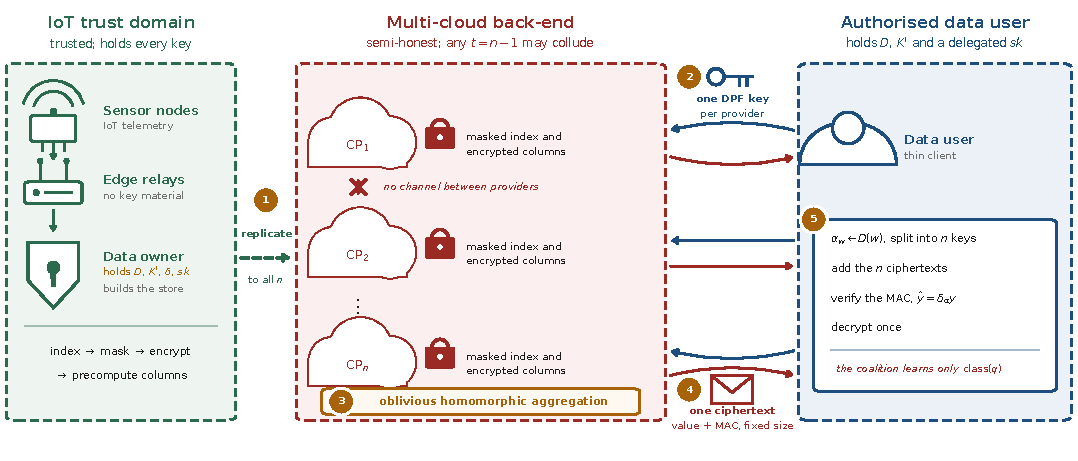
\includegraphics[width=\textwidth]{figures/fig_architecture.pdf}
\caption{Overview of CR-SHE. The owner replicates a masked index and encrypted
columns to $n$ clouds (1). A query is split into DPF keys, one set per cloud
(2); each cloud aggregates obliviously over its own share (3) and returns one
ciphertext carrying value and check value (4); the user combines, verifies and
decrypts (5). No cloud sees the matched set or its size. Drawn by a plotting
script written with the assistance of a generative AI tool (see the
declaration before the references).}
\label{fig:arch}
\end{figure*}

\emph{Threat model.} The adversary is probabilistic polynomial-time, static
and semi-honest: it corrupts a coalition $C$ of at most $t=n-1$ providers,
which follow the protocol and pool everything they see, over adaptively chosen
queries. The goal is that this view be simulatable from data-independent
leakage that reveals neither the keyword or range, the access pattern, the
result-set size nor the result. The DO and authorised DUs are honest, channels
are authenticated and confidential, and side channels beyond message sizes are
out of scope. Beyond this goal we address two active threats:
\emph{deviating providers}, which may return any response at all
(Section~\ref{sec:verify}), and \emph{users exceeding their authority}, who
may send malformed keys or arbitrary share vectors (Section~\ref{sec:auth}).
Collusion between a DU and a provider is excluded, since the DU already holds
decryption capability.

\emph{Primitives.} A pseudorandom function (PRF) $F$ has distinguishing
advantage $\advPRF$ against a random function \citep{goldreich2019construct}.
An $n$-party DPF \citep{gilboa2014distributed,boyle2015function,boyle2016function}
for point functions $f_{\alpha,\beta}:[N]\to\mathbb{Z}_p$ is a pair
$(\Gen,\Eval)$ with correctness $\sum_j\Eval(j,\kappa_j,x)=f_{\alpha,\beta}(x)$
and $(n{-}1)$-privacy: the keys of any $n-1$ parties are simulatable without
$(\alpha,\beta)$, up to $\advDPF$. The two-party construction has keys of
$O(\lambda\log N)$ bits and full-domain evaluation in $O(N)$ PRG calls; for
$n>2$ we use the additive sharing of a unit vector in which $n-1$ parties hold
seeds and one an explicit vector. Leveled BFV
\citep{fan2012somewhat,cryptoeprint:2016/421} over plaintext ring
$\mathbb{Z}_p$ is IND-CPA with advantage $\advCPA$; we write $\bplus$ for
ciphertext addition and $\bdot$ for plaintext-ciphertext multiplication, and
use $\ell$ SIMD slots arranged in two rows of $\ell/2$
\citep{halevi2014algorithms}. Table~\ref{tab:notation} lists the notation.

\begin{table}[pos=htbp]
\caption{Notation.}
\label{tab:notation}
\centering
\footnotesize
\begin{tabular}{@{}ll@{}}
\toprule
Symbol & Meaning \\
\midrule
$n,\ t$ & number of providers; collusion bound $t=n-1$ \\
$N,\ N_d$ & tag domain size; number of records \\
$p,\ \ell$ & plaintext modulus and DPF output group; SIMD slots \\
$I,\ I',\ P$ & membership index; masked index; one-time pad \\
$\alpha_w,\ \kappa_j,\ e_j$ & row of keyword $w$; key of $\text{CP}_j$; its full-domain evaluation \\
$m_i,\ w_f$ & value of record $i$; weights of template $f$ \\
$A_f$ & aggregate column of template $f$ over the tag domain \\
$d,\ M$ & cube dimension; number of cells $\prod_k s_k$ \\
$C_f,\ T_f$ & cell aggregates; their summed-area table \\
$\kappa_\sigma(B),\ \beta_\sigma$ & corner $\sigma\in\{0,1\}^d$ of box $B$; its sign or $0$ \\
$\delta_s$ & per-query secret of the tamper check, uniform on $\mathbb{Z}_p^{*}$ \\
$\rho,\ K'_\rho$ & role; its mask key \\
$S,\ |S|$ & matched record set; its size \\
\bottomrule
\end{tabular}
\end{table}

% ===========================================================================
\section{The CR-SHE construction}
\label{sec:construction}

\subsection{Overview, and why a homomorphic layer}
\label{sec:whyrep}
The DO builds a membership index $I\in\{0,1\}^{N\times N_d}$ in which keyword
$w$ occupies row $\alpha_w=D(w)$ of a secret, append-only dictionary, stores it
masked (Section~\ref{sec:mask}), and encrypts aggregate columns, cube tables
and the record column under $pk$ (Algorithm~\ref{alg:setup}). Rather than
recovering the selection and asking providers to aggregate over the named
records, which hands them $S$, each provider contracts its own share of the
selection against encrypted data (Algorithm~\ref{alg:query}).

The obvious alternative, dealing the data as an $(n,n)$ additive sharing and
answering DPF queries over the shares, fails under our constraints.

\begin{proposition}[No local answers over shares]
\label{prop:nolocal}
Let a column $A\in\mathbb{Z}_p^N$ be dealt as $A=\sum_{k\in[n]}S_k$ with
$S_1,\dots,S_{n-1}$ uniform, and let $e_j$ be the evaluation vector of the DPF
key $\kappa_j$ for $f_{\alpha,1}$. If each provider returns
$r_j=\langle e_j,S_j\rangle$, then
$\sum_j r_j-A[\alpha]=-\sum_{j\neq k}\langle e_j,S_k\rangle$, and for $n=2$ this
error is uniform on $\mathbb{Z}_p$ except with negligible probability.
\end{proposition}
\begin{pf}
$A[\alpha]=\sum_{j,k}\langle e_j,S_k\rangle$ and the answers supply only the
diagonal. For $n=2$, substituting $S_2=A-S_1$ gives the error
$-\langle e_1,A\rangle+\langle e_1-e_2,S_1\rangle$, uniform since $S_1$ is
uniform and independent of the keys whenever $e_1\neq e_2$; $e_1=e_2$ would let
a provider read $\alpha$ from its own key, so it has negligible probability by
DPF privacy. \qed
\end{pf}

The cross terms are not an artefact of linear answers. In any non-interactive
scheme where a provider holds an additive share, queries are formed without
reference to the data, and the scheme is correct on every share tuple, a client
holding a database $X$ at a single server can set that server's share to $X$,
play the other providers itself and subtract their contributions; this yields
single-server PIR, which implies oblivious transfer
\citep{dicrescenzo2000single} and is instantiated by homomorphic encryption
\citep{kushilevitz1997replication}. Within that class, sharing the data moves
the public-key primitive into a per-share PIR rather than removing it; a lower
threshold ($t<n/2$, as in Obscure), interaction or preprocessing escapes the
argument (Supplementary S1). Replicas under one owner key also survive the
loss of $n-1$ providers, keep answering over any surviving pair, and let the
owner add or revoke a provider by copying ciphertexts.

\subsection{Oblivious homomorphic aggregation}
\label{sec:oha}
Suppose the providers hold additive shares $v_1,\dots,v_n\in\mathbb{Z}_p^M$ of
a vector $v$ and replicas of an encrypted column
$\mathrm{C}=(\Enc_{pk}(c_1),\dots,\Enc_{pk}(c_M))$. Provider $j$ returns
\begin{equation}
\label{eq:contract}
\text{ct}_j=\bplus_{i\in[M]} v_j[i]\bdot\mathrm{C}_i ,
\end{equation}
and $\bplus_j\text{ct}_j$ decrypts to $\langle v,c\rangle$. Nothing that leaves
a provider depends on $v$ beyond its own share, and the response is one
ciphertext of fixed size whatever the support of $v$.

\begin{lemma}[Algebraic compatibility]
\label{lem:compat}
If the DPF output group and the plaintext ring are the same $\mathbb{Z}_p$ and
$\sum_i|v[i]\,c_i|<p$, then the contraction~\eqref{eq:contract} summed over the
providers decrypts to $\sum_i v[i]\,c_i$ over the integers.
\end{lemma}
\begin{pf}
$\bdot$ and $\bplus$ are homomorphisms over the same ring, so summation
commutes with decryption; the magnitude bound prevents wraparound. Decryption
correctness is a noise-budget question: a plaintext-ciphertext product by a
uniform share in $\mathbb{Z}_p$ scales the noise by up to $p\approx2^{36}$
without consuming a level, which the parameters must absorb; we check the worst
case empirically (Section~\ref{sec:correctness}). \qed
\end{pf}
Instantiating the DPF over $\mathbb{Z}_{2^k}$ and the homomorphic scheme over
an unrelated modulus, the natural default when the two libraries are chosen
independently, silently breaks correctness through wraparound.

\subsection{The masked, packed index}
\label{sec:mask}
Stored in the clear, the index would hand every provider each posting-list
length, which the attack of Section~\ref{sec:leakeval} turns into tag
identities. As DORY does for its Bloom-filter bits \citep{dory}, the DO stores
it one-time-padded, here with field-element masks that arithmetic DPF shares
can strip, and packed $\pi=32$ membership bits per word:
\begin{equation}
\label{eq:mask}
I'[x][c]=\textstyle\sum_{b<\pi}I[x][\pi c+b]\,2^b+P[x][c]\bmod p ,
\end{equation}
where $P[x][c]$ is drawn from $F'_{K'}(x,c)$ by rejection sampling: a 37-bit
candidate is kept only if it is below $p$, so each mask word is exactly
uniform. A packed word is below $2^{32}<p$, so the pad hides it perfectly, and
the index shrinks 32-fold; the four spare bits of each word catch a uniformly
corrupted word except with probability $1/16$.

\begin{theorem}[Index hiding]
\label{thm:mask}
For any two indexes $I_0,I_1$, no $\PPT$ distinguisher tells
$\mathrm{pack}(I_0)+P$ from $\mathrm{pack}(I_1)+P$ with advantage greater than
$\advPRF_{F'}$; the stored index reveals no posting-list length and no
membership relation.
\end{theorem}
\begin{pf}
With $F'$ replaced by a random function, rejection sampling makes every mask
word independent and exactly uniform on $\mathbb{Z}_p$, so
$\mathrm{pack}(I_b)+P$ is a one-time pad for either $b$. \qed
\end{pf}
Reducing 64-bit words modulo $p$ instead biases each mask word by
$r(p-r)/(p\,2^{64})\approx8.27\times10^{-10}$, $r=2^{64}\bmod p$; over the
$146{,}625{,}960$ words of the packed telemetry index the union bound is about
$0.12$, so rejection sampling is what makes Theorem~\ref{thm:mask} hold as
stated.

\subsection{Single-keyword aggregates and the packed response}
\label{sec:fast}
For an aggregate over one keyword's posting list under a template registered
at setup, the DO precomputes $A_f[x]=\sum_i I[x][i]\,w_f[i]\,m_i$ for every
tag $x$ and encrypts it as packed ciphertexts. A query is one DPF key per
provider for $f_{\alpha_w,1}$, and~\eqref{eq:contract} with $v_j=e_j$ over
$A_f$ costs $O(N)$ PRG calls and $O(N/\ell)$ plaintext-ciphertext products,
independent of $N_d$. The DO places $A_f$ in slot row~0 and its check column
in row~1, chunked $\ell/2$ tags per ciphertext; the provider multiplies each
chunk by its evaluation vector, adds the chunks and rotates and sums within
the rows, so slot~0 carries the value share and slot $\ell/2$ the check share
in one ciphertext. With $k$ templates each row is cut into $k$ segments, so
one ciphertext answers, for instance, a count and a sum (a mean) or a count,
sum and sum of squares (a variance). Modulus switching to one RNS tower halves
the response. Conjunctions and weights chosen at query time use a two-round
flexible path (Section~\ref{sec:auth}).

\subsection{Oblivious range aggregation over data cubes}
\label{sec:range}
\emph{Data cubes.} The DO registers a cube of $d$ ordered tag families of sizes
$s_1,\dots,s_d$, for example device, one-minute window and the decile band of
one sensor, such that each record $i$ falls in exactly one cell
$c(i)\in\prod_k[s_k]$. For each template $f$ it computes the cell aggregates
$C_f[c]=\sum_{i:\,c(i)=c}w_f[i]\,m_i$ and the summed-area table
$T_f[c]=\sum_{c'\le c}C_f[c']$, with $\le$ coordinate-wise, flattened into a
column of $M=\prod_ks_k$ entries and encrypted like $A_f$.

\emph{Queries.} For a box $B=\prod_k[\mathit{lo}_k,\mathit{hi}_k]$ and
$\sigma\in\{0,1\}^d$, let corner $\kappa_\sigma(B)$ take $\mathit{lo}_k-1$ on
the axes where $\sigma_k=1$ and $\mathit{hi}_k$ elsewhere. By
inclusion--exclusion,
\begin{equation}
\label{eq:ie}
\sum_{c\in B}C_f[c]=\sum_{\sigma\in\{0,1\}^d}(-1)^{|\sigma|}\,T_f[\kappa_\sigma(B)],
\end{equation}
where a corner with a coordinate $-1$ lies outside the cube and contributes
$0$. The DU sends, for every $\sigma$, one DPF key per provider for the point
$\kappa_\sigma(B)$ with output $\beta_\sigma=(-1)^{|\sigma|}\bmod p$, and for a
corner outside the cube a \emph{dummy} key with $\beta_\sigma=0$ at a random
point. DPF keys hide $\beta$ as well as the point, so every query to a cube
carries exactly $2^d$ indistinguishable keys per provider, and a box at the
cube's edge cannot be told from an interior one.

\emph{Answering.} Provider $j$ evaluates its $2^d$ keys over all $M$ cells,
adds them, $e_j=\sum_\sigma e_{\sigma,j}$, and contracts once against the
encrypted table; the response is one ciphertext, and the DU decrypts the box
aggregate in slot~0 (Algorithm~\ref{alg:query}). The cost per provider is
$2^d$ full-domain evaluations over $M$ cells, $\lceil kM/(\ell/2)\rceil$
plaintext-ciphertext products for $k$ templates and $\log_2(\ell/2k)$
rotations; the uplink is $2^d$ keys of $O(\lambda\log M)$ bits. Nothing depends
on the box or on $N_d$; Lemma~\ref{lem:compat} requires the cube's total to stay
below $p$.

\emph{Why prefix sums rather than interval keys.} Function secret sharing for
$d$-dimensional intervals \citep{boyle2016function} needs the servers to hold
each record's coordinates, but over owner-encrypted records the coordinates
(which device, which minute, which band) are the sensitive part. A dense,
encrypted table over all $M$ cells keeps them hidden and lets each of the
$2^d$ pieces be a point function; the price is that cubes are registered and
precomputed, at a cost that grows with $M$ rather than with the record count.

\begin{algorithm}[t]
\footnotesize
\caption{Outsourcing at the data owner.}
\label{alg:setup}
\begin{algorithmic}[1]
\Require records $i\in[N_d]$ with tags, values $m_i$ and roles $\rho(i)\in[R]$;
  templates $\{w_f\}$; cubes $(\mathcal{F}_1,\dots,\mathcal{F}_d)$
\State $(pk,sk)\gets\mathsf{KGen}(1^\lambda,p,\ell)$; \ $K'\gets\{0,1\}^\lambda$; \ $D\gets\emptyset$
\ForAll{keywords $w$ in arrival order}
  \State \textbf{if} $w\notin D$ \textbf{then} $D(w)\gets|D|$ \Comment{rows never move}
\EndFor
\State $I[D(w)][i]\gets1$ for every keyword $w$ of record $i$
\State $K'_\rho\gets F_{K'}(\rho)$ for every role $\rho$
\State $P[x][c]\gets$ rejection-sampled $F'_{K'_{\rho(c)}}(x,c)$, uniform on $\mathbb{Z}_p$
\State $I'\gets\mathrm{pack}_{32}(I)+P \bmod p$ \Comment{masked, packed index}
\ForAll{roles $\rho$ and templates $f$}
  \State $A^{\rho}_f[x]\gets\sum_{i:\rho(i)=\rho} I[x][i]\,w_f[i]\,m_i$ for $x\in[N]$
  \State $C^{\rho}_f[c]\gets\sum_{i:\,c(i)=c,\,\rho(i)=\rho} w_f[i]\,m_i$; \ $T^{\rho}_f[c]\gets\sum_{c'\le c}C^{\rho}_f[c']$
  \State pack $A^{\rho}_f$, $T^{\rho}_f$ and the record column in slot row 0,
  \Statex \hspace{\algorithmicindent} with a copy in row 1, and encrypt under $pk$
\EndFor
\State \Return $I'$, ciphertexts and $pk$ to every $\text{CP}_j$;
  \ $(sk, D, K'_\rho)$ to the data users of role $\rho$
\end{algorithmic}

\end{algorithm}

\begin{algorithm}[t]
\footnotesize
\caption{Verified range query. A single-keyword aggregate is the case $d=0$:
one key pair at $\alpha_w$ over $A_f$.}
\label{alg:query}
\begin{algorithmic}[1]
\Statex \textbf{Token} at the data user, for box $B$ of a registered cube
\State $\delta_s\gets\mathbb{Z}_p^{*}$ \Comment{fresh per query}
\ForAll{$\sigma\in\{0,1\}^d$}
  \State $c\gets\kappa_\sigma(B)$; \ $\beta\gets(-1)^{|\sigma|}$
  \State \textbf{if} $c$ lies outside the cube \textbf{then} $c\gets$ random cell, $\beta\gets0$ \Comment{dummy}
  \State $(\kappa_{\sigma,1},\dots,\kappa_{\sigma,n})\gets\Gen(1^\lambda,c,\beta)$
  \State $(\hat\kappa_{\sigma,1},\dots,\hat\kappa_{\sigma,n})\gets\Gen(1^\lambda,c,\delta_s\beta)$
\EndFor
\State send $\{\kappa_{\sigma,j},\hat\kappa_{\sigma,j}\}_\sigma$ to $\text{CP}_j$
\Statex \textbf{Answer} at provider $\text{CP}_j$
\State $e_j\gets\sum_\sigma\mathsf{FullEval}(j,\kappa_{\sigma,j})$; \
  $\hat e_j\gets\sum_\sigma\mathsf{FullEval}(j,\hat\kappa_{\sigma,j})$ \Comment{$O(2^dM)$ PRG}
\State $\text{ct}_j\gets\bplus_c E_{j,c}\bdot T_c$, \ $E_{j,c}$: chunk $c$ of $e_j$ in row 0, of $\hat e_j$ in row 1
\State rotate and sum within segments; modulus-switch; \Return $\text{ct}_j$ \Comment{one ciphertext}
\Statex \textbf{Combine} at the data user
\State $(y,\hat y)\gets$ slots $(0,\ell/2)$ of $\Dec\big(sk,\bplus_j\text{ct}_j\big)$
\State \textbf{if} $\hat y\neq\delta_s y$ \textbf{then abort} \Comment{tamper evidence}
\State \Return $y$
\end{algorithmic}

\end{algorithm}

\subsection{Tamper evidence}
\label{sec:verify}
Every response carries a second slot row, so a check value travels with the
answer at no extra downlink. A single stored MAC key, row~1 holding $\delta
m_i$, catches inconsistent responses but not a provider that applies the same
substitution to both rows, for instance contracting against $k\,e_j$, which
shifts value and tag in the ratio $\delta$. Per-position keys
$\delta_x=F''_{K''}(x)$ catch substitutions spread over other positions but
not one concentrated on the queried position, and do not exist for
contractions over records.

\emph{A per-query secret.} The session layout stores no key at all: row~1 of
every column and table is a copy of row~0. With each query the DU draws a
fresh $\delta_s$ uniformly from $\mathbb{Z}_p^{*}$ and sends a second key set
for the same points with outputs multiplied by $\delta_s$
($\delta_s\beta_\sigma$ at each corner of a range, fresh shares of
$\delta_sv$ in a flexible round). Each provider places the second evaluation
vector in row~1 of the same plaintexts, so the homomorphic work is unchanged
and slot $\ell/2$ decrypts to $\delta_sy$; the DU accepts only if
$\hat y=\delta_sy$.

\begin{theorem}[Tamper evidence]
\label{thm:tamper}
Consider one query in the session layout. Let a coalition of at most $n-1$
providers return arbitrary responses computed from its members' views, with at
least one honest provider, an honest DU that keeps $\delta_s$ secret, and no
provider colluding with the DU. The DU accepts an output $y'\neq y$, where $y$
is the honest answer, with probability at most
\[
\frac{1}{p-1}+\varepsilon ,
\]
where $\varepsilon=\kappa\,\advDPF$ for a query with $\kappa$ DPF keys per
provider in its $\delta_s$-carrying set ($\kappa=1$ for a keyword or a
retrieval, $2^d$ for a range) and $\varepsilon=\advPRF$ for a flexible round.
Over $Q$ queries the bounds add.
\end{theorem}
\begin{pf}[Proof sketch]
Let $(r_0,r_1)$ be what the coalition's responses decrypt to in the two slots
and $(y_C,\hat y_C)$ what its members would have contributed honestly; all are
functions of the coalition's view $V$. The DU decrypts $y'=y-y_C+r_0$ and
$\hat y'=\delta_sy-\hat y_C+r_1$ and accepts if and only if
$r_1-\hat y_C=\delta_s(y'-y)$. Replacing the coalition's $\delta_s$-carrying
keys by keys for an independent scalar changes the probability of this event by
at most $\kappa\,\advDPF$, since DPF privacy hides the output as well as the
point. Then $V$ is independent of $\delta_s$, and since $y'-y\neq0$ at most one
of the $p-1$ equally likely values of $\delta_s$ satisfies the equation. Each
query draws a fresh $\delta_s$, so a union bound covers $Q$ adaptive queries
(full proof in Supplementary S2). \qed
\end{pf}
The bound puts no restriction on how a provider deviates: it may rescale the
queried point, swap or mix slot rows, replay an old response or return any
ciphertext. It does not guarantee output delivery, and a DU that reveals its
aborts can leak up to one bit about the data per query, which retrying silently
through another provider set avoids.

\subsection{Retrieval, flexible queries and role-scoped access}
\label{sec:auth}
\emph{Retrieval.} Providers return $b_j=\sum_x e_j[x]\,I'[x]$; the DU adds the
shares, subtracts $P[\alpha_w]$, which it derives from its mask key, and
unpacks the posting list. The response is $\lceil N_d/32\rceil$ words whatever
$|S|$, and payloads are fetched with a batch of DPF retrievals padded to a
public bound.

\emph{Flexible queries.} For a conjunction, a disjunction or weights chosen at
query time, the DU first retrieves the posting lists, forms the selection
vector $v$ over the records, deals it as fresh additive shares (seeds to $n-1$
providers, an explicit vector to one) and has each provider
contract~\eqref{eq:contract} against the record column. Every share a
coalition holds is uniform or pseudorandom, so the second round reveals
nothing about $v$; the DU learns $S$, which it already knows.

\emph{Role-scoped access.} DPF privacy hides the queried row, so no provider can
check \emph{which} keyword or range a query targets, and a user who sends
arbitrary share vectors can read every linear function of the columns it
reaches. We therefore restrict what the columns and keys cover. The DO assigns
each record a role $\rho(i)$, lays out record identifiers so that each packed
word holds records of one role, derives $K'_\rho=F_{K'}(\rho)$ and masks word
$c$ under $K'_{\rho(c)}$, and builds $A^{\rho}_f$, $T^{\rho}_f$ and the record
column from role $\rho$'s records only. A provider answers a role-$\rho$ user
from role $\rho$'s columns, selected by the user's authenticated identity; it
needs no exchange with other providers.

\begin{proposition}[Role confinement]
\label{prop:role}
If every provider authenticates the user's role and applies that role's
columns on every path, and no provider colludes with the user, then the view of
a role-$\rho$ user, for any queries including malformed keys and arbitrary
share vectors, is simulatable from role $\rho$'s records and the public
dimensions, up to $\advPRF$.
\end{proposition}
\begin{pf}
Aggregate, range and flexible responses are linear in role-$\rho$ columns.
Retrieval returns linear combinations of masked words; words of other roles
carry masks under keys $K'_{\rho'}$ the user lacks, which become one-time pads
once $F$ is replaced by a random function. \qed
\end{pf}
The mechanism costs storage per role rather than interaction, reveals each
query's role to the providers, and does not express rights finer than a record
partition.

% ===========================================================================
\section{Security analysis}
\label{sec:security}

\emph{Leakage.} The setup leakage $\Leak_{\mathrm{Setup}}$ is what a provider
sees in its replica: $(n,t,N,N_d,p,\ell)$, the registered templates and
ciphertext shapes, the cubes' dimensions $(s_1,\dots,s_d)$, the number of roles
and their spans of packed words, and tier sizes. The per-query leakage to the
providers is $\Leak^{\text{CP}}_{\mathrm{Query}}=\mathrm{class}(q)$: whether a
query is a keyword aggregate, a range over a named cube, a retrieval or a
flexible round, the user's role, and whether it carries the verification key
set. It contains no keyword, range, access pattern, result size or result, and
by Theorem~\ref{thm:mask} the setup leakage contains no posting-list length.

\begin{definition}[$\Leak$-security against $t$-collusion]
\label{def:sec}
In $\Real$, the adversary picks a database and a coalition $C$ with $|C|\le t$,
receives the coalition's stored state, and adaptively issues $Q$ queries,
receiving after each the coalition's keys or shares and the responses those
providers compute. In $\Ideal$, a simulator produces the same views from
$\Leak_{\mathrm{Setup}}$ and $\mathrm{class}(q)$ alone. CR-SHE is
$\Leak$-adaptively-secure if for every $\PPT$ adversary some $\PPT$ simulator
makes the two experiments indistinguishable up to $\negl(\lambda)$.
\end{definition}

\begin{theorem}[Correctness]
\label{thm:correct}
For templates and cubes satisfying the magnitude bound of
Lemma~\ref{lem:compat}, a keyword aggregate returns $\sum_{i\in S}w_f[i]\,m_i$,
a range query on box $B$ returns $\sum_{i:\,c(i)\in B}w_f[i]\,m_i$, a retrieval
returns exactly $S$, and a flexible round on $v$ returns $\sum_iv[i]\,m_i$,
except with the negligible probability that decryption fails; honest
responses always pass the check.
\end{theorem}
\begin{pf}[Proof sketch]
DPF correctness gives $\sum_je_j=u_{\alpha_w}$ for a keyword and
$\sum_\sigma\beta_\sigma u_{\kappa_\sigma}$ for a range, so by
Lemma~\ref{lem:compat} the sum of responses decrypts to $A_f[\alpha_w]$, or to
$\sum_\sigma\beta_\sigma T_f[\kappa_\sigma]$, which~\eqref{eq:ie} turns into
the box aggregate; the true value lies in $[0,p)$, so the reduction modulo $p$
loses nothing although individual signed terms are negative. Rotations act
within slot rows, so templates and check values do not mix, and row~1 decrypts
to $\delta_s$ times row~0 for honest providers (Supplementary S3). \qed
\end{pf}

\begin{theorem}[$t$-collusion leakage security]
\label{thm:sec}
If $F$ and $F'$ are secure PRFs, $(\Gen,\Eval)$ is an $(n{-}1)$-private DPF and
the homomorphic and symmetric schemes are IND-CPA, then CR-SHE is
$\Leak$-adaptively-secure against $t=n-1$ colluding providers, with
\[
\big|\Pr[\Real=1]-\Pr[\Ideal=1]\big|\le\advPRF_{F'}
+Q\big(2^{d_{\max}+1}\advDPF+2\,\advPRF\big)+m\,\advCPA ,
\]
where $d_{\max}$ is the largest registered cube dimension and $m$ the number of
ciphertexts in the coalition's view.
\end{theorem}
\begin{pf}[Proof sketch]
A sequence of hybrids replaces (1) $F'$ by a random function, after which the
masked index is a one-time pad of the all-zero index (Theorem~\ref{thm:mask});
(2) every DPF key the coalition holds, dummies and $\delta_s$-carrying keys
included, by simulated keys, which hide both point and output; (3) flexible
shares by uniform vectors; and (4) every stored ciphertext by an encryption of
$0$. Each response is a deterministic function of the provider's keys or shares,
the query class and its stored state, so the simulator recomputes it. The final
hybrid depends only on the leakage (Supplementary S4). As is standard for BFV,
IND-CPA is assumed to hold given the rotation keys. \qed
\end{pf}

Recovering $S$ and then asking providers to aggregate over it would put $S$
itself, a function of the query and the database, in the coalition's view,
which no simulator given data-independent leakage can produce. What makes
Theorem~\ref{thm:sec} hold is contracting a share at the provider, not the
number of rounds. Because providers never interact and receive only keys or
shares, a deviating coalition sees the same view, so deviation buys it no
information about the query, and Theorem~\ref{thm:tamper} makes any
answer-changing deviation evident.

% ===========================================================================
\section{Implementation and experimental setup}
\label{sec:impl}
Two implementations share the parameters below. A C++17 prototype implements
the single-keyword path; it produced the single-keyword measurements on the
real datasets. An open reference implementation (Python driving OpenFHE's C++
kernels) implements the full construction: range aggregation in the
\emph{combined} (one key set, no check), \emph{verified} (session check) and
\emph{per-corner} (per-cell keys) layouts, all three verification modes on
every path, role-scoped columns and mask keys, the packed masked index with
rejection-sampled masks, retrieval, the flexible path, and a single-server
baseline. Its 83 tests include DPF checks at every point of every domain up to
depth 8, range answers against brute force for $d\le3$ and $n\le3$, and failure
controls that must and do fail, such as a flipped corner sign or a provider
told $\delta_s$.

\emph{Parameters.} The two-party DPF is the Boyle--Gilboa--Ishai GGM-tree
construction \citep{boyle2016function} with fixed-key AES-128. The homomorphic
layer is leveled BFV in OpenFHE \citep{openfhe} at plaintext modulus
$p=68{,}724{,}326{,}401$, a 37-bit prime with $p\equiv1\bmod2^{17}$, ring
dimension $8{,}192$, multiplicative depth 1, at the 128-bit security level. In
both implementations the DPF output group and the plaintext ring are one
modulus object, so the error Lemma~\ref{lem:compat} warns about cannot be
written.

\emph{Datasets.} The Environmental Sensor Telemetry dataset
\citep{stafford_2020_environmental} has $405{,}184$ messages from three sensor
arrays, indexed under device, one-minute window, decile bands of five sensor
channels and two flags: $N=11{,}580$ tags over $3{,}646{,}656$ postings. The
UCI Beijing Multi-Site Air-Quality dataset
\citep{zhang2017cautionary,chen2019beijing} has $420{,}370$ hourly records from
twelve sites after dropping those without a temperature, $N=35{,}162$ tags over
$4{,}624{,}070$ postings. Both aggregate temperature in hundredths of a degree.

\emph{Machines.} C++: an AMD EPYC 7J13 with 64 cores, medians of 11 runs.
Reference implementation: synthetic-data runs on a cloud VM with four vCPUs of
an Intel Xeon at 2.1\,GHz; real-dataset runs on an AMD EPYC 7J13 server with 32
vCPUs; one thread, medians of 5--21 runs. Every table is generated from the
result files by a script, and latencies from different machines are not
compared with each other.

% ===========================================================================
\section{Results and discussion}
\label{sec:results}

\subsection{Correctness}
\label{sec:correctness}
On both real datasets the reference implementation matched the plaintext
ground truth for 200 random tags at each $n\in\{2,3,4\}$ on the keyword,
retrieval and flexible paths, all $1{,}800$ queries per dataset correct, with a
$132{,}081$\,B response throughout, and every range query below decrypted to
the plaintext box aggregate. The C++ prototype matched the ground truth for
$1{,}000$ random tags per template and $n\in\{2,3,4\}$ on both datasets and
sent a byte-identical response for matched sets of size 0 and $4{,}999$.

\subsection{Range aggregation on real data}
\label{sec:rangeresult}
We built two cubes from the records themselves: device $\times$ one-minute
window $\times$ CO band over the telemetry data ($M=345{,}690$ cells) and site
$\times$ day $\times$ PM$_{2.5}$ band over the Beijing data, with missing
readings as an eleventh band ($M=192{,}852$). A query fixes one device or site,
a window of $L$ minutes or days and bands 3--7, so $d=3$ and each provider
receives 8 keys, or 16 verified. Table~\ref{tab:rangereal} reports the
per-provider cost.

\begin{table}[pos=htbp]
\caption{Range aggregation per provider on cubes built from the real datasets,
against window length $L$; $d=3$, two templates. Every query returns
$132{,}081$\,B; uplink per provider is $2{,}760$ and $2{,}624$\,B combined,
$5{,}520$ and $5{,}248$\,B verified.}
\label{tab:rangereal}
\centering
\footnotesize
\begin{tabular*}{\tblwidth}{@{\extracolsep{\fill}}lccc@{}}
\toprule
$L$ & Combined total (ms) & Verified: DPF eval (ms) & Verified total (ms) \\
\midrule
\inputtbl tables/range_real.tex
\bottomrule
\end{tabular*}
\end{table}

\emph{Cost does not depend on the range.} A verified query costs $1.19$\,s per
provider on the telemetry cube and $0.68$--$0.77$\,s on the Beijing cube, and a
combined query $0.77$--$0.79$\,s and $0.44$--$0.48$\,s, with no trend in $L$
from one window to the whole timeline. A box at the cube's origin, with seven
of its eight corners dummies, costs the same ($1{,}192.6$ and $758.9$\,ms
verified). Every response is one $132{,}081$\,B ciphertext, and the data user
spends $1.1$--$1.9$\,ms combining, checking and decrypting.

\emph{Verification costs one key set, not a layout.} The verified layout
stores the same ciphertexts as the combined one, a copy of the table in place
of a MAC row, and performs the same homomorphic products; it adds a second set
of keys and its full-domain evaluation. On a synthetic cube of the same
dimensions it costs $1.6$--$1.9$ times the combined layout and less than half
the per-corner layout ($3.24$--$3.44$\,s), which stores the table eight times
and still misses deviations at the queried corner (Supplementary S5). Range
cost grows linearly with the cube: $34.7$, $129.3$ and $1{,}356.0$\,ms per
provider for $10^4$, about $10^5$ and $10^6$ cells in the combined layout, so
cube size, not record count or range length, is what a deployment provisions.

\emph{The trust split pays on the uplink.} A single server holding the same
encrypted tables needs no non-collusion assumption but an encrypted query as
long as the table: $44.4$\,MB and $25.0$\,MB for the two cubes (computed from
the measured ciphertext size), against $5.5$ and $5.2$\,kB of DPF keys per
provider verified, four orders of magnitude, which is the regime of a thin or
metered IoT client. Answering the same box through single-tag aggregates would
need one query per cell, $1{,}200$ for a 240-minute window over five bands,
revealing the box's size.

\subsection{Tamper evidence}
\label{sec:verifyresult}
Table~\ref{tab:verify} injects five provider deviations, 200 trials each, into
every path and verification mode; one provider deviates and the other is
honest. The last deviation is the strongest we can stage: the provider
perturbs exactly the point the query reads, as if it knew the query.

\begin{table}[pos=htbp]
\caption{Detected / undetected-and-wrong over 200 trials per cell. Deviations:
a constant added to the value slot; the share plus a uniform vector; the share
scaled by $k$; the share plus $c\,u_x$ at a random point; the same at the
queried point. Trials not counted were undetected but left the answer correct
(the perturbed row was empty).}
\label{tab:verify}
\centering
\footnotesize
\setlength{\tabcolsep}{3pt}
\begin{tabular*}{\tblwidth}{@{\extracolsep{\fill}}llccccc@{}}
\toprule
Path & Check & Constant & Uniform & Scale & Random pt & Queried pt \\
\midrule
\inputtbl tables/verify.tex
\bottomrule
\end{tabular*}
\end{table}

A single stored key catches only the inconsistent constant: every consistent
substitution was accepted with a wrong answer on every path. Per-position keys
catch every deviation except the one aimed at the queried point, which passed
200 times out of 200 on the keyword and range paths. The session check
detected every deviation that changed the answer: across the $4{,}000$ session
trials no wrong answer was accepted. On both real cubes it also flagged all 250
tampered range queries (five deviations, fifty each), while the combined layout
without a check returned 200 of them wrong and unflagged.

\subsection{Single-keyword aggregates and baselines}
\label{sec:aggresult}
In the C++ prototype a keyword aggregate costs $38.8$--$39.2$\,ms per provider
across a $405\times$ range of record counts, $N_d=10^3$ to $405{,}184$, because
the precomputed column removes $N_d$ from the query. Table~\ref{tab:baselines}
places it against baselines on the telemetry data for a tag with the median
$|S|=35$. The DORY-style search-only baseline costs $3.3\times$ more because it
materialises the selection vector; a faithful homomorphic equality scan needs
depth 17 and costs $617\times$ more, consistent with the fifteen hours HADES
reports for a million encrypted records.

\begin{table}[pos=htbp]
\caption{Single-keyword aggregate against baselines, telemetry data,
$N_d=10^5$, C++, median $|S|=35$; $\dagger$ marks an extrapolated value.}
\label{tab:baselines}
\centering
\footnotesize
\setlength{\tabcolsep}{3pt}
\begin{tabular}{@{}lccl@{}}
\toprule
System & Server (ms) & Downlink (B) & Leakage to the server(s) \\
\midrule
Plaintext scan & $<0.001$ & $8$ & everything \\
SSE, 1 server & $<0.001$ & $560$ & search and access pattern, $|S|$ \\
Path ORAM & $0.059^{\dagger}$ & $373{,}248$ & $|S|$, via access count \\
DORY-style search & $130.4$ & $800{,}000$ & none; no analytics \\
FHE equality scan & $24{,}157^{\dagger}$ & n/a & none; 1 server \\
\midrule
\textbf{CR-SHE, keyword} & $\mathbf{39.2}$ & $\mathbf{525{,}950}$ & $\mathrm{class}(q)$ only \\
\bottomrule
\end{tabular}
\end{table}

In the reference implementation the packed response halves provider work and
downlink: a single template falls from $53.0$ to $23.5$\,ms at $N=11{,}580$,
and four templates fit in one compressed $132{,}081$\,B ciphertext in
$32.7$\,ms, against $194.9$\,ms and $2{,}104{,}088$\,B for four unpacked
responses. A single server holding the same columns (baseline vi) costs $42.6$
and $92.5$\,ms at the two tag domains, $1.8$ and $2.9$ times one CR-SHE
provider, but two providers together spend $47.0$ and $62.8$\,ms, so in total
server work the trust split is not cheaper. Its case rests on the client: the
single server's query is $789{,}033$ and $2{,}367{,}099$\,B of fresh
ciphertexts against a $260$ or $294$\,B DPF key per provider, and $14.6$ and
$67.5$\,ms of client encryption against $0.54$ and $0.62$\,ms of key
generation.

\subsection{Leakage evaluation}
\label{sec:leakeval}
We mount a frequency and volume leakage-abuse attack
\citep{islam2012access,cash2015leakage} against four representations of the
index: unmasked, whose rows expose every posting-list length; padded to the
next power of two; volume-hiding, every row padded to the longest; and the
masked index~\eqref{eq:mask}, with row statistics computed under the real PRF.
The adversary's auxiliary knowledge is the tag frequencies of a similar
deployment, modelled by thinning the true lengths to a fraction $f$ of the
records; it assigns each row to the tag of nearest auxiliary frequency,
breaking ties at random (Fig.~\ref{fig:leakage}, Table~\ref{tab:leakage}).

\begin{figure}[pos=htbp]
\centering
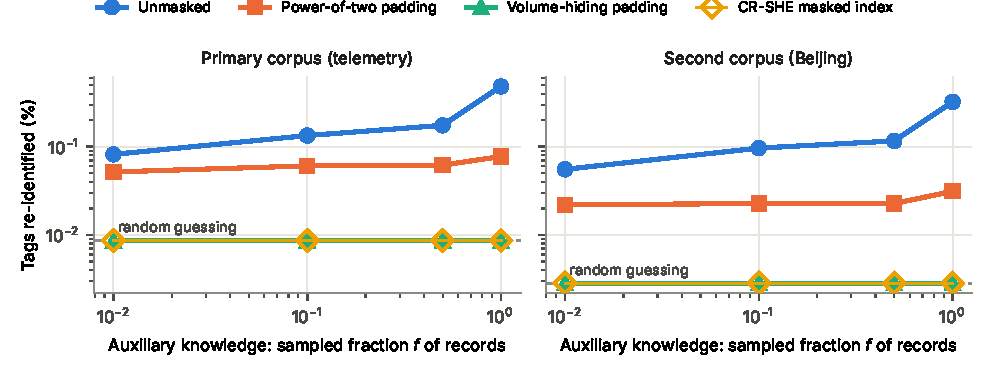
\includegraphics[width=\linewidth]{figures/fig_leakage_reference.pdf}
\caption{Share of tags re-identified against the adversary's auxiliary
knowledge, four index representations, both datasets (log scales). The
volume-hiding and masked curves coincide with random guessing. Plotted from the
measured results by a script written with the assistance of a generative AI
tool (see the declaration before the references).}
\label{fig:leakage}
\end{figure}

\begin{table}[pos=htbp]
\caption{Tag re-identification by class under perfect auxiliary knowledge
($f=1$). In the masked column the attack's guesses all fall on the longest
posting list, so one tag per dataset is matched by default.}
\label{tab:leakage}
\centering
\footnotesize
\setlength{\tabcolsep}{3pt}
\begin{tabular*}{\tblwidth}{@{\extracolsep{\fill}}lcccc@{}}
\toprule
Tag class & Unmasked & Power of two & Volume-hiding & Masked \\
\midrule
\inputtbl tables/leakage_real.tex
\bottomrule
\end{tabular*}
\end{table}

\emph{Unmasked, the index gives away the tags that carry meaning:} every
device, flag, temperature band and wind direction, and $92.5$--$100\%$ of most
band families. At $f=1$ a tag is missed only when another tag has exactly the
same length, and the attack then reaches the best any length-only attacker
can do: $0.484\%$ and $0.324\%$ overall, $56\times$ and $114\times$ random
guessing, low only because time buckets of near-identical length dominate the
tag universe. \emph{Power-of-two padding}, at $1.55\times$ and $1.54\times$
storage, still re-identifies $9\times$ and $11\times$ random guessing, and
$75\%$ of the motion flags. \emph{Volume-hiding padding and the masked index}
both reduce the attack to random guessing at every $f$ on both datasets, but
volume hiding inflates postings $1{,}285\times$ and $752\times$, while the
packed masked index costs $2\times$ a plaintext bitmap. Higher figures from an
earlier run in our C++ prototype exceed this length-only bound and are
withdrawn (Supplementary S6).

\subsection{Role-scoped access and deployment}
\label{sec:authresult}
A role-0 user sending raw shares for all 512 rows of an index over three roles
of $4{,}096$ records recovered every row, including all $365{,}227$ membership
bits of the other roles, when one mask key was used, and none of those bits
with role-scoped keys; $6.06\%$ of the other roles' words passed the width
check under its own key, against the $6.25\%$ expected of uniform words. With
$n\in\{2,3,4\}$ provider processes over loopback, provider compute was flat in
$n$, $34.82$--$35.48$\,ms, and end-to-end latency rose from $44.1$ to
$52.5$\,ms in transport alone.

% ===========================================================================
\section{Discussion and limitations}
\label{sec:limits}
\emph{Ranges are where the design pays.} A registered range aggregate costs
the same for a one-minute window as for a four-year timeline and returns one
ciphertext, where single-tag aggregates need one query per cell and a single
server an encrypted query as long as the cube. The per-query secret removes the
old choice between a cheap unverifiable layout and an expensive per-corner one.

\emph{Scope of the evaluation.} Range aggregation, the session check and
role-scoped access run in a single-threaded reference implementation, so
absolute latencies are those of an unoptimised driver; the C++ prototype covers
the single-keyword path. The deployment ran over loopback, so wide-area
latency and stragglers were not measured. No system in
Table~\ref{tab:compare} was run on the same data and hardware.

\emph{Expressiveness and adversary.} One-round ranges apply to registered cubes
whose total stays below $p$; other predicates use the two-round flexible path,
and cube updates are not implemented. Privacy is proved for semi-honest
providers; tamper evidence covers arbitrary deviation without output delivery,
and role confinement assumes providers enforce the policy. For $n>2$ our DPF is
non-succinct, so key-size claims are for $n=2$.

\emph{Prior art.} The $2^d$ box decomposition \citep{boyle2016function}, the
one-time-padded index \citep{dory} and the client-chosen one-time MAC key
\citep{li2026silent} each have a precursor; our contribution is their
composition into one-round, verifiable range analytics over owner-encrypted
replicas at $t=n-1$.

% ===========================================================================
\section{Conclusion}
\label{sec:conclusion}
IoT analytics are range aggregates over time, place and value, and the data
behind them increasingly sit encrypted across several clouds. CR-SHE answers
such aggregates in one round over data encrypted under one owner's key, hiding
the range, the matched records, their number and the result from any coalition
of up to $n-1$ clouds that never communicate. Encrypted summed-area tables turn
any box into $2^d$ padded point keys, oblivious homomorphic aggregation keeps
the matched set from ever being assembled, a secret scalar drawn per query
makes tampering evident at no extra homomorphic cost, and role-scoped columns
confine each user to its own records. On two real IoT datasets a verified
range query costs $0.68$--$1.19$\,s per cloud with a fixed $132$\,kB response
and kilobytes of upload, no tampered answer was accepted, and a frequency
attack fell to random guessing where power-of-two padding did not. Future work
will port the range path to native code, evaluate cross-region deployments,
add succinct multi-party DPFs for $n>2$ and support multiple data owners.

\section*{Supplementary material}
The Supplementary Material (PDF) accompanies this article: S1, the full
argument for a homomorphic layer at $t=n-1$; S2, the stored-key verification
modes and the full proof of Theorem~\ref{thm:tamper}; S3 and S4, the full
proofs of Theorems~\ref{thm:correct} and~\ref{thm:sec}; S5, dynamic ingest, the
complexity table and further measurements (range layouts and cube size,
selection latency, packing and the single-server baseline, the flexible path,
the packed index, deployment, communication, setup and scaling, role
extraction and the second dataset in the C++ prototype); and S6, the withdrawn
leakage figures of an earlier C++ run.


\ifanonymous\else\printcredits\fi

%%DECLARATIONS%%
\section*{Declaration of competing interest}
The authors declare that they have no known competing financial interests or
personal relationships that could have appeared to influence the work reported
in this paper.

\section*{Funding}
This research did not receive any specific grant from funding agencies in the
public, commercial, or not-for-profit sectors.

\section*{Data availability}
The two datasets are public (Kaggle, Environmental Sensor Telemetry Data; UCI
Machine Learning Repository, Beijing Multi-Site Air-Quality Data). The
reference implementation, benchmark scripts and result files will be made
available on request.

\section*{Declaration of generative AI and AI-assisted technologies in the
manuscript preparation process}
During the preparation of this work the authors used three AI assistants.
Claude (Anthropic) was used to develop the reference implementation with its
tests and benchmark scripts, search and compare the literature, draft and edit
parts of the text and analysis, including the range construction, the
tamper-evidence mechanism, role-scoped access and their proofs, condense the
manuscript to its present length, and convert it to the journal's format.
ChatGPT (OpenAI) and Gemini (Google) were used to edit and review intermediate
drafts; changes adopted from them were checked against the implementation and
the measured results. No image was generated or altered by a generative AI
tool. After using these tools, the authors reviewed and edited the content as
needed and take full responsibility for the content of the publication.
%%END%%

\bibliographystyle{model1-num-names}
\bibliography{references}

\end{document}
